%\vspace{-0.05in}
\section{Introduction}
%\vspace{-0.05in}
%GPUs have enabled parallel processing for not just graphics applications but
%for a wide range of HPC installations and data-centers like Amazon's elastic
%compute cloud (EC2).  With this massively parallel processing often comes an
%insatiable demand for main memory bandwidth as GPUs churn through data at an
%ever increasing rate.  To meet this bandwidth demand, many GPUs have been
%designed with attached high-bandwidth GDDR memory rather than standard DDR
%memory used by CPUs.  As a result, many GPUs today have GDDR bandwidth that is
%2-5$\times$ higher than the memory bandwidth available to the CPU in the
%system.  To make best use of the bandwidth available to GPU programs
%programmers manually copy the data over the relatively slow PCIe bus to the GPU
%memory, and -- only then -- launch their GPU kernels.  This up-front data
%allocation and transfer has been necessary since transferring data over the
%PCIe bus is a high overhead operation, and a bulk transfer of data amortizes
%this overhead. This data manipulation overhead also results in significant
%porting challenges when retargeting existing applications to GPUs, particularly
%for high-level languages that make use of libraries and dynamic memory
%allocation during application execution.
%
%\begin{figure}[t]
%    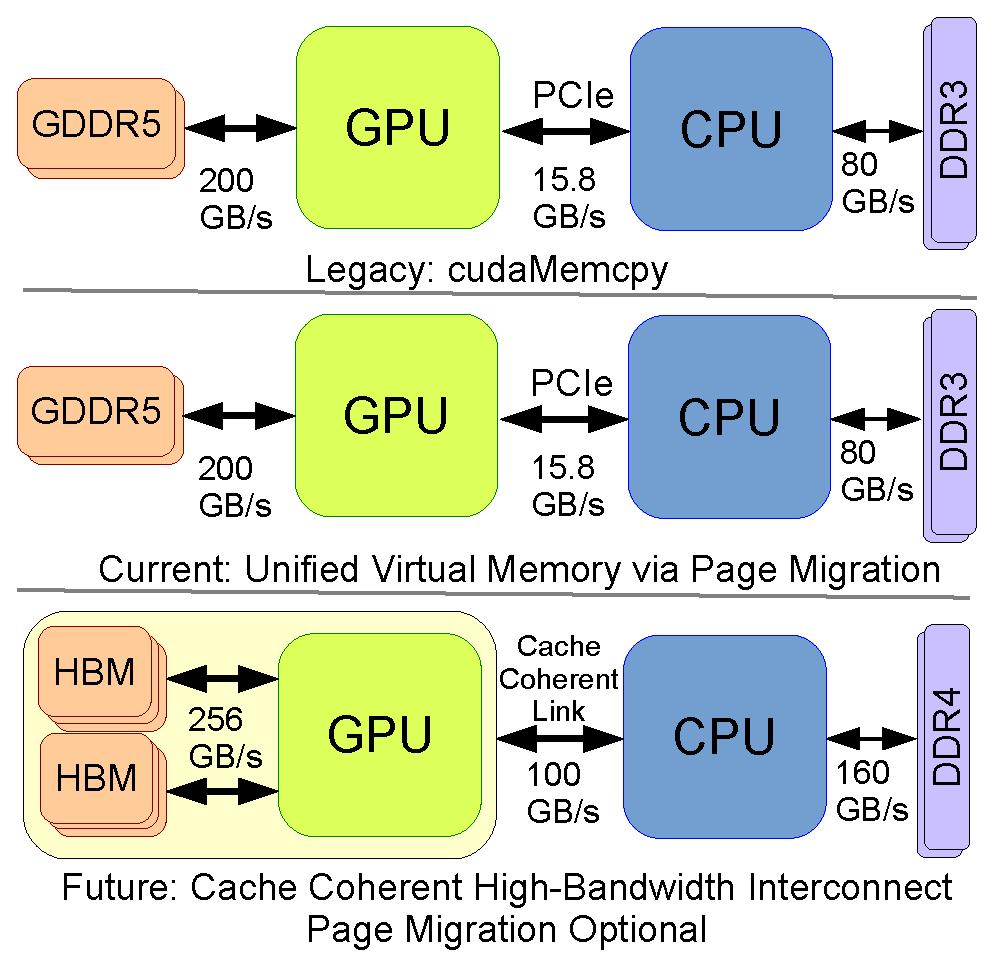
\includegraphics[width=\columnwidth]{hpca2015/figures/architecture.eps}
%    \caption{System architectures for legacy, current, and future mixed GPU-CPU systems.}
%    \label{fig:arch}
%\end{figure}
%
%Recognizing the obstacle this programming model poses to the wider adoption of
%GPUs in more parallel applications, programming systems like NVIDIA's CUDA,
%OpenCL, and OpenACC are evolving. Concurrently, GPU-CPU architectures are
%evolving to have unified globally addressable memory systems in which both the
%GPU and CPU can access any portion of memory at any time, regardless of its
%physical location.  Today this unified view of memory is layered on top of
%legacy hardware designs by implementing software-based runtimes that
%dynamically copy data on demand between the GPU and CPU~\cite{cuda}. As
%depicted in Figure~\ref{fig:arch}, over the next several years it is expected
%that GPU and CPU systems will move away from the PCIe interface to a fully
%cache coherent (CC) interface ~\cite{AMDHSA}. These systems will provide high
%bandwidth and low latency between the non-uniform memory access (NUMA) pools
%attached to discrete processors by layering coherence protocols on top of
%physical link technologies such as NVLink~\cite{NVLINK},
%Hypertransport~\cite{AMDHT}, or QPI~\cite{INTELQPI}.   CC-NUMA access to host
%memory from the GPU makes the software page migration used today an optional
%feature thanks to the improved bandwidth, latency, and access granularity that
%cache coherence can provides.
%
GPUs are throughput oriented processors that spawn thousands of threads
concurrently, demanding high memory bandwidth. To maximize the bandwidth
utilization programmers copy over the data to high bandwidth memory like GDDR5
before launching GPU kernels to amortize the overhead of accessing memory over
microsecond link latencies like PCIe. Hence, it is the responsibility of the
programmer to identify data that will be accessed by the GPU and copy it over to
the GPU-attached high bandwidth memory. NVIDIA's unified virtual
memory~\cite{UVM} has relaxed this constraint to enhance GPU programmability by
providing a software mechanism that performs on demand {\tt memcpy} of the data
as GPU accesses it. However, on demand data copying hurts GPU throughput. In
this chapter we discuss techniques of performing programmer agnostic dynamic
memory migration of performance critical data across CC-NUMA CPU-GPU system
connected by a next generation interconnect technology to maximize bandwidth
utilization, while not demanding the programmer to perform explicitly {\tt
memcpy(s)}.  We specifically examine how to best balance accesses through
cache-coherence and page migration.

%The contributions of this work are the following:

%While interconnect advancements improve GPU-CPU connectivity, no reduction is
%expected in the memory bandwidth differential between CPU and GPU-attached
%memory.  On-package memories such as High Bandwidth Memory (HBM) or Wide-IO2
%(WIO2) may in fact increase this differential as GPU bandwidth requirement
%continues to grow, feeding the ever increasing number of parallel cores
%available on GPUs used by both graphics and compute workloads. On the other
%hand, architects will likely continue to balance latency, power, and cost
%constraints against raw bandwidth improvement for CPU attached memory, where
%bandwidth and application performance are less strongly correlated. With
%application data residing primarily in CPU memory on application start-up, the
%GPU can access this memory either via hardware cache-coherence (which improves
%memory system transparency to the programmer) or by migrating a memory page into
%GPU physical memory (facilitating greater peak bandwidth for future requests).
%In this work we specifically examine how to best balance accesses through
%cache-coherence and page migration for a hypothetical CC-NUMA GPU-CPU system
%connected by a next generation interconnect technology.  The contributions of
%this work are the following:

%\begin{enumerate}
%\item
%1) Counter-based metrics to determine when to migrate pages from the CPU to GPU 
%are insufficient for finding an optimal migration policy to exploit GPU memory bandwidth. 
%In streaming workloads, where each page
%may be accessed only a few times, waiting for $N$ accesses to occur before
%migrating a page will actually limit the number of accesses that occur after
%migration, reducing the efficacy of the page migration operation.

%\item
%2) TLB shootdown and refill overhead can significantly degrade the
%performance of any page migration policy for GPUs\@. We show that combining reactive
%migration with virtual address locality information to aggressively prefetch pages
%can mitigate much of this overhead, resulting in increased GPU throughput.

%\item
%3) The legacy intuition to migrate all data to the GPU local memory in an attempt to maximize bandwidth fails to leverage
%the bandwidth available via the new CC-NUMA interface.  A page migration policy which 
%is aware of this differential and balances migration with CC-NUMA link
%utilization will outperform either GPU or GPU memory being used in isolation.

%\item 
%4) We present a software based memory placement system that, on average, outperforms CC-NUMA based
%accesses by 1.95$\times$, performs 6\% better than the legacy CPU to GPU {\tt
%memcpy} approach by 
%intelligently using both CPU and GPU memory bandwidth, and comes within 28\% of oracular page placement,
%all while maintaining the relaxed memory semantics of modern GPUs.
%\end{enumerate}
